\section{Probenherstellung und Messmethoden}\label{sec:messmethoden}

\subsection{Gepulste Laserabscheidung}\label{subsec:pld}
\begin{figure}
    \centering
    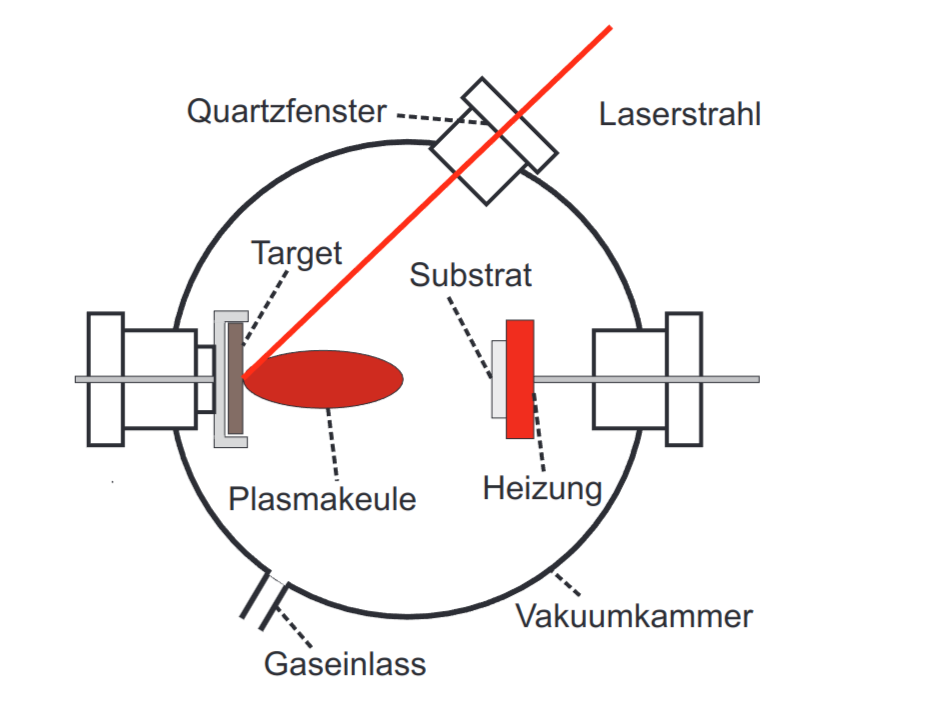
\includegraphics[width=0.6\textwidth]{../assets/messmethoden/pld/aufbau}
    \caption{Schematischer Aufbau eines PLD-Systems.}
    \label{fig:pld}
\end{figure}
Die im Rahmen dieser Arbeit betrachteten Dünnfilme wurden mithilfe der gepulsten Laserabscheidung
(PLD, engl. \textit{pulsed laser deposition}) hergestellt.
Dafür wird ein hochenergetischer, gepulster Laserstrahl auf ein Target in einer Vakuumkammer abgebildet, welches bei
hinreichender, materialabhängiger Energie beginnt zu schmelzen und zu verdampfen.
Durch die Wechselwirkung der herausgelösten Atome mit den Laserpulsen entsteht eine Plasmawolke, die sich senkrecht
zum Target ausbreitet.
Die Plasmawolke expandiert in der Vakuumkammer und kann auf einem passend platzierten Substrat abgeschieden werden.
Der schematische Aufbau eines PLD-Systems ist in \cref{fig:pld} dargestellt.
Im Folgenden soll dieser Mechanismus genauer beschrieben werden.

Bevor ein PLD Prozess gestartet werden kann, muss ein geeignetes Target ausgewählt werden.
Dieses besteht aus dem Material, aus dem der Dünnfilm hergestellt werden soll.
Für die Arbeit wurde von Jorrit Bredow ein \heo-Target hergestellt.
Für die \heo-Proben wurden die Binäroxidpulver im äquimolaren Verhältnis abgewogen, in einer Kugelmühle gemahlen,
in eine zylindrische Form gepresst und anschließend für \qty{12}{\hour} bei \qty{1000}{\celsius} gesintert.
Danach kann es im Targethalter montiert werden.

Der gesamte Prozess findet in einer Vakuumkammer statt, um den Druck und das Hintergrundgas während des PLD Prozesses zu
kontrollieren.
Durch Vor- und Turbomolekularpumpen kann ein Vakuum in der Größenordnung von \qty{e-4}{\milli\bar} erzeugt werden.
Zusätzlich können auch Hintergrundgase, unter anderem Sauerstoff und Stickstoff, in die Kammer eingelassen werden.

Um einen PLD Prozess zu starten, muss vorher das Hintergrundgas und dessen Druck in der Vakuumkammer eingestellt werden.
Außerhalb der Vakuumkammer generiert ein \ce{KrF}-Excimerlaser mit einer Wellenlänge von \qty{248}{\nano\meter}
Laserpulse mit einer Energie von \qty{650}{\milli\joule} und einer Pulsdauer von \qty{20}{\nano\second}.
Diese Laserpulse werden durch ein Fenster in die Vakuumkammer geleitet und auf das Target abgebildet.
Die Laserpulse werden vom Target absorbiert und führen zu elektronischen Anregungen, die durch
Elektron-Phonon-Wechselwirkung in thermische, chemische und mechanische Energie umgewandelt werden.
Das führt zur Erhitzung des Targets, welches schmilzt und verdampft.
Da das Target durch den Laserstrahl nur an einer kleinen Stelle erhitzt wird, ist es notwendig,
dass sich das Target relativ zum Laserstrahl bewegt, um eine gleichmäßige Abtragung zu gewährleisten.
Um das zu gewährleisten wird eine Tranlationsbewegung des Targets relativ zum Laserstrahl durchgeführt.
Hinzu kommt eine Rotation des Targets, um eine gleichmäßige Abtragung zu gewährleisten.

Mithilfe der oben genannten Komponenten kann der Abscheidungsprozess durchgeführt werden.
Die Laserphotonen treffen auf das Target und regen dort Elektronen an.
Diese erfahren einen Intraband-Übergang, wodurch sie in einen angeregten Zustand übergehen.
Durch die Elektron-Phonon-Wechselwirkung relaxiert das Elektron und gibt dabei Energie in Form von Phononen ab.
Dies führt zur Erhitzung des Targets, welche nicht nur an der Oberfläche, sondern auch im Inneren stattfindet.
Durch die hohe Temperatur beginnt das Target zu Verdampfen.

Die verdampften Atome interagieren ebenfalls mit den Laserphotonen und bilden eine Plasmawolke, die sich in der
Vakuumkammer ausbreitet.
Die Plasmawolke expandiert in der Vakuumkammer senkrecht zum Target.
Das Hintergrungas in der Vakuumkammer beeinflusst die Plasmawolke durch Stoßprozesse.

Gegenüber vom Target befindet sich der Substrathalter, auf dem das Substrat montiert wird.
Hinzu kommt ein Substrathalter, auf dem das Substrat montiert wird.
Für die Arbeit wurden Eagle-XG-Glassubstrate und C-Saphirsubstrate verwendet.
Dieses kann durch einen Widerstandsheizer auf eine Temperatur von bis zu \qty{800}{\celsius} beziehungsweise
mithilfe eines Laserheizers auf circa \qty{1100}{\celsius} erhitzt werden.
Das Substrat selbst hat üblicherweise die Maße von circa \qty{10}{\milli\meter\squared}.

Auch die verdampften Konstituenten des Targets wechselwirken mit den Laserphotonen.
Durch Photoionisation werden Elektronen herausgelöst, sodass eine Plasmawolke entsteht.
Diese breitet sich in der Vakuumkammer in Richtung Substrat aus und beginnt sich auf dem diesem abzusetzen.
Durch Adsorptionsprozesse beginnt die Bildung eines Dünnfilms.\autocite[2299-2301]{pld}

Die hier betrachteten Dünnfilmproben wurden bei Raumtemperatur und unterschiedlichen Drücken in Sauerstoffatmosphäre
auf $\qty{10}{\milli\meter} \times \qty{10}{\milli\meter}$  Corning Eagle XG Glassubstraten abgeschieden.]

\subsection{Ausheizmethoden}\label{subsec:ausheiz}

Dabei ist es wichtig, den Temperaturbereich von \qty{600}{\degreeCelsius} bis \qty{1000}{\degreeCelsius} zu erreichen
und die Temperatur des Dünnfilms möglichst genau zu bestimmen.
Ein geeigneter Kandidat für diesen Prozess ist die A-Kammer, die mithilfe eines Heizlasers die Rückseite des
Substrathalters erhitzt.
Um die Temperatur des Dünnfilms zu bestimmen, wird ein Pyrometer verwendet, welches die Rückseite des Substrathalters
misst.
Mithilfe eines PID-Reglers wird die Temperatur auf den eingestellten Wert geregelt.

\newpage

\subsection{XRD}\label{subsec:xrd}
Nachdem die Dünnfilme hergestellt wurden, ist der nächste Schritt, ihre Struktur zu charakterisieren.
Zwischen Dünnfilmen und ihren korrespondierenden Massivkörpern existieren signifikante Unterschiede.
Diese resultieren vorrangig aus dem Verhältnis von Oberfläche zu Volumen, sowie den jeweiligen
Wachstumsbedingungen, wie Temperatur, Druck und Substrat.
Sie zeigen sich beispielsweise in der Qualität der Kristallinität, sowie in Kompositionsgradienten.
Da Proben mit unterschiedlichen Wachstumsbedingungen hergestellt wurden und deren Eigenschaften dadurch
maßgeblich beeinflusst werden, ist es notwendig, die Kristallinität der Dünnfilme zu charakterisieren.
Röntgendiffraktometrie (XRD, engl. \textit{X-Ray diffraction}) ist eine weit verbreitete Methode, um die
Kristallstruktur von Dünnfilmen zu bestimmen.
Dabei wird ein Röntgendiffraktometer verwendet.

\subsubsection{Röntgendiffraktometer}
Das Röntgendiffraktometer besteht aus fünf Hauptkomponenten: Röntgenquelle und Detektor, Ein- und Ausfallsoptik,
sowie dem Goniometer.
Zusätzlich ist das Diffraktometer durch eine Strahlungsschutzverkleidung abgeschirmt und mit einer Steuerungssoftware
verbunden.
Im Folgenden werden die einzelnen Komponenten näher erläutert.

\paragraph{Röntgenquelle}
Die Röntgenstrahlen werden in einer Röntgenröhre erzeugt.
In dieser werden Elektronen aus einer Wolfram-Glühkathode emittiert und durch das elektrische Feld auf eine Anode
beschleunigt.
Die Anode besteht meist aus hochreinem Kupfer.
Stromstärke und Beschleunigungsspannung der Röntgenröhre müssen so gewählt werden, dass die Energie beim Auftreffen der
Elektronen auf die Anode ausreicht, um die gebundenen Elektronen der Atome auf das nächsthöhere Energieniveau anzuregen.
Aufgrund der daraus resultierende Wärme muss die Anode ständig wassergekühlt werden.
Im hauseigenen Röntgendiffraktometer wird eine Beschleunigungsspannung von \qty{40}{\kilo\volt} und eine Stromstärke
von \qty{40}{\milli\ampere} verwendet.

Nach der Kollision zwischen Kupferatom und Elektron relaxiert das Elektron unter Bildung eines Röntgenphotons.
Man erhält ein Spektrum, welches durch die charakteristische Strahlung der Anode sowie durch Bremsstrahlung
geprägt ist.
Die charakteristische Strahlung wird vorrangig durch die K-Linien, insbesondere $K_{\alpha_1}$, $K_{\alpha_2}$
und K$_{\beta}$, dominiert.
Da $K_{\alpha_1}$ und $K_{\alpha_2}$ energetisch sehr nahe beieinander liegen, können sie nicht immer einzeln
aufgelöst werden.
Die $K_{\beta}$ Strahlung ist größtenteils unerwünscht und kann durch geeignete Filter unterdrückt werden.

Die Wolfram-Glühkathode emittiert unerwünschterweise nicht nur Elektronen, sondern auch Wolfram-Atome in kleinen Mengen.
Über längere Zeiträume führt dies zu einer nicht mehr zu vernachlässigenden Kontamination der Anode.
Dadurch können bei Elektronenstößen auch Wolfram-Atome angeregt werden, was zu einer zusätzlichen Wellenlänge im
Spektrum führt
In den späteren Messergebnissen sind diese Beiträge erkennbar.
Abschließend gelangen die Röntgenstrahlen durch ein Berylliumfenster in die Einfallsoptik.

\paragraph{Goniometer}
Das Goniometer ist die mechanische Komponente des Röntgendiffraktometers.
Es besteht aus mehreren Drehachsen, die es ermöglichen, die Probe in unterschiedlichsten Winkeln auszurichten.
Nach der Braggschen Beugungstheorie ergeben sich konstruktive Interferenzen an denjenigen Winkeln, die der
Bragg-Bedingung genügen.
Existieren Möglichkeit, die Winkel für Quelle und Detektor zu variieren, kann diese Interferenz beobachtet werden.
Im Allgemeinen ist die Röntgenquelle jedoch fest, eine äquivalente Drehung von Probe und Detektor ist deshalb gängig.
In der einfachsten Betrachtungsweise muss das Goniometer also den Winkel zwischen Probe und Quelle ($\omega$) und dem
Winkel zwischen Probe und Detektor ($2\theta$) einstellen können.
Diese Freiheit reicht zwar für Pulverproben, jedoch nicht für Dünnfilme.
Zwar kann man mit beiden Freiheitsgraden Messungen durchführen, welche die out-of-plane Orientierung charakterisieren,
jedoch ist es nicht möglich, die in-plane Orientierung zu bestimmen.
Dafür werden weitere Achsen, wie $\varphi$ und $\chi$, benötigt.
Eine Konstruktion mit den vier Achsen wird Euler-Wiege genannt.

\paragraph{Ein- und Ausfallsoptik}
Es existieren zwei primäre Möglichkeiten, um den Strahlengang zwischen Quelle, Probe und Detektor zu modifizieren:
Bragg-Brentano-Geometrie und parallele Geometrie.
In der Bragg-Brentano-Geometrie wird ein hochintensiver, divergierender Röntgenstrahl auf die Probe gerichtet,
welcher unter Ausnutzung bestimmter Geometrien zurück auf den Detektor fokussiert werden kann.
Aufgrund der Divergenz des Strahls ist diese Methode fehleranfällig und gerade für $\varphi$ und $\omega$ scans
ist eine Parallelstrahloptik, wie in \cref{fig:xrd_parallel} gezeigt, von Vorteil.
\begin{figure}
    \centering
    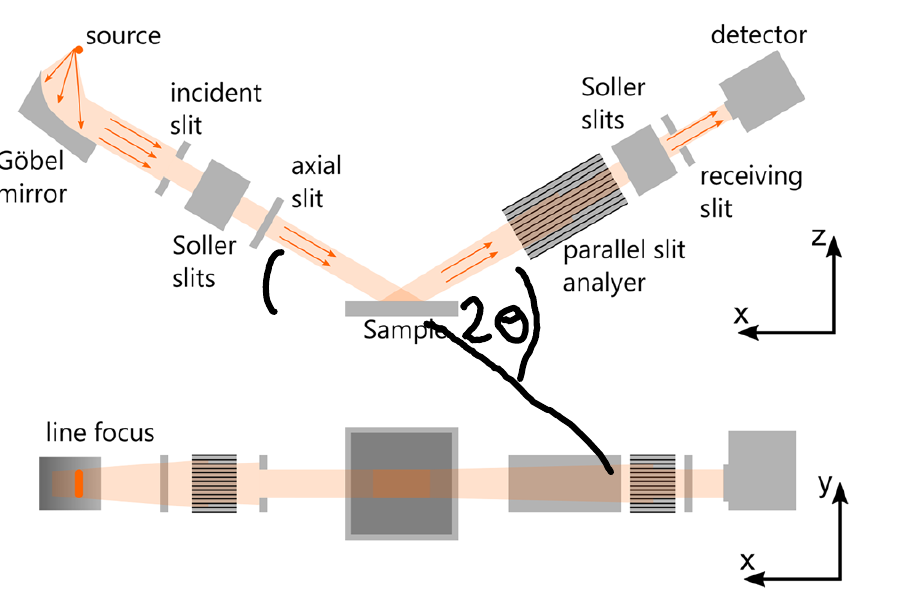
\includegraphics[width=0.6\textwidth]{../assets/messmethoden/xrd/paralleloptik}
    \caption{Aufbau der Parallelstrahloptik \imcitetwo[146]{btb-xrd}}
    \label{fig:xrd_parallel}
\end{figure}
Die aus der Quelle austretenden divergierenden Strahlen werden durch einen Göbel-Spiegel
parallelisiert und durchlaufen anschließend einen Eingangs- und Axialspalt, die den Winkelbereich
festlegen.
Dazwischen liegt ein Soller Spalt, der die Divergenz in axialer Richtung begrenzt, da diese
nicht durch den Göbel-Spiegel eliminiert werden kann.
Anschließend reflektiert der Strahl an der Probe und gelangt über weitere Spalte zum Detektor.

\paragraph{Detektor}
Der Röntgendetektor dient dazu, die Intensität der reflektierten Röntgenstrahlen zu messen und
in elektrische Signale umzuwandeln.
Im hauseigenen Röntgendiffraktometer wird ein Halbleiterdetektor verwendet
Die Grundidee eines Halbleiterdetektors ist, das Material durch Photonen zu ionisieren und dabei freie Ladungsträger zu
erzeugen.
Diese werden über ein elektrisches Feld extrahiert und elektronisch gezählt.
Durch die matrixartige Anordnung einzelner Halbleiterzellen kann die Intensität in Abhängigkeit der Position bestimmt
werden.
Somit können unterschiedliche Detektormodi realisiert werden, wie 0D Punktdetektion,
1D Linien- oder 2D Flächendetektion.
Wichtig ist, dass die maximale Zählrate des Detektors nicht überschritten wird.
Das führt zu nicht linearen Antworten und kann den Sensor beschädigen.
Um das zu vermeiden, können Filter und Attenuatoren verwendet werden.

\subsubsection{Scanmethoden}
Durch den hohen Freiheitsgrad des Goniometers können unterschiedliche Scanmethoden realisiert werden.
Diejenigen, die in dieser Arbeit verwendet wurden, sind im Folgenden beschrieben.

\paragraph{$2\theta/\omega$ scan}
Ein $2\theta/\omega$ scan ist eine einfache Methode, um die Kristallstruktur von Dünnfilmen zu bestimmen
und bildet die Grundlage für weitere Messungen.
Die Probe wird auf den Probenhalter montiert und in das Goniometer eingesetzt.
Der Winkel zwischen Probenoberfläche und Quelle wird als $\omega$ und der Winkel zwischen Probenoberfläche und Detektor
als $2\theta$ bezeichnet.
Als Anfangsbedingung legt man Messdauer und ein Intervall für $\omega$ fest und startet die Messung.
Nun fahren Goniometer und Detektor über den angegebenen Winkelbereich mit der Bedingung $\omega = \theta$.
Als Ausgabe bekommt man ein Intensitätsprofil in Abhängigkeit von $2\theta$, in denen im Idealfall charakteristische
Peaks erkennbar sind.
Diese Peaks entstammen der Bragg-Reflexion von Kristallebenen, die parallel zur Probenoberfläche liegen.
Kennt man die Wellenlänge der Röntgenstrahlung, so kann mam mithilfe des Peaks den Gitterabstand bestimmen.
Somit ist es möglich, Rückschlüsse auf die vorhandenen Kristallstrukturen im Dünnfilm zu ziehen.

\paragraph{$\omega$ scan}

\paragraph{$\varphi$ scan}
%%TODO
\newpage

\subsection{Rasterkraftmikroskopie}\label{subsec:afm}
Mithilfe der Rasterkraftmikroskopie (AFM, engl. \textit{Atomic Force Microscopy}) kann die Oberflächenstruktur der
Dünnfilme charakterisiert werden.
Das Rasterkraftmikroskop ist ein hochpräzises Messinstrument zum Erfassen von Oberflächenstrukturen.
Anders als bei Licht- oder Elektronenmikroskopie wird hierbei eine mechanische Funktionsweise verwendet.
Dabei fährt der Cantilever, eine Messnadel, rasterweise über eine Oberfläche und tastet diese ab.
Die Spitze des Cantilevers ist im Nanometerbereich dimensioniert und kann so auch kleinste Strukturen erfassen.
Die auf den Cantilever wirkenden interatomaren oder magnetischen Kräfte führen zu messbaren Auslenkungen,
woraus eine Topographiekarte der Oberfläche erstellt wird.
Das in der Arbeit benutzte Rasterkraftmikroskop ist das \textit{XE-150} von Park Systems.
In den folgenden Abschnitten wird der Aufbau und die Funktionsweise des Rasterkraftmikroskops
erläutert, basierend auf den Erkenntnissen von \citeauthoryear{afm-buch} \autocite{afm-buch}.

\subsubsection{Schematischer Aufbau und Funktionsweise}
\begin{figure}
    \centering
    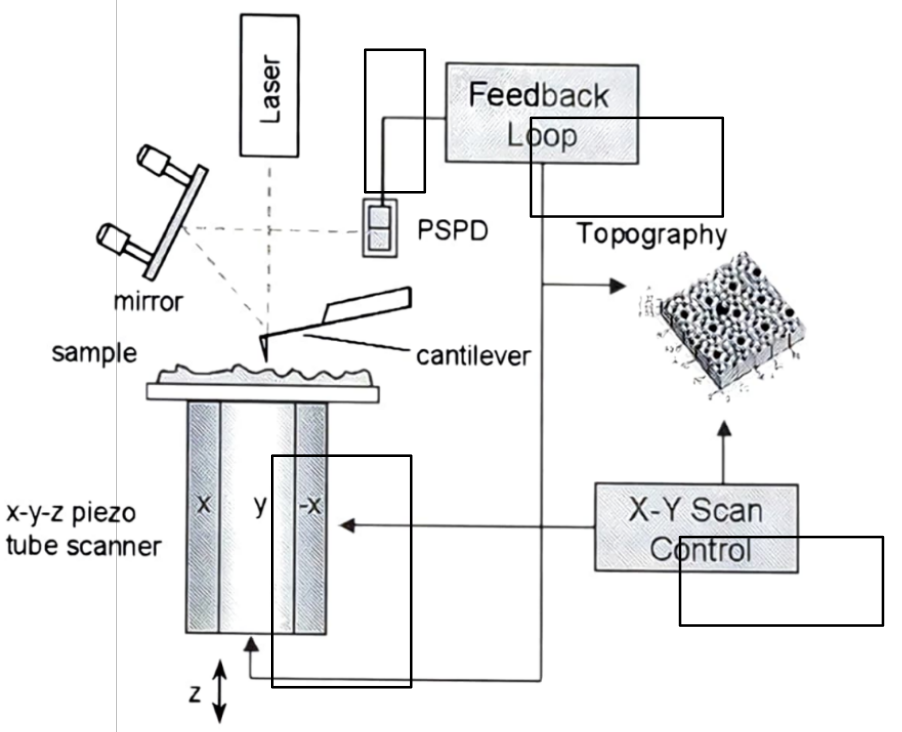
\includegraphics[width=0.6\textwidth]{../assets/messmethoden/afm/01_aufbau}
    \caption{Schematischer Aufbau eines Rasterkraftmikroskops. \imcite{afm-buch}}
    \label{fig:afm_aufbau}
\end{figure}
Die grundlegende Funktionsweise ist in \cref{fig:afm_aufbau} dargestellt.
Fährt der Cantilever über die Probe, so wirken interatomare Kräfte auf die Spitze, welche den Cantilever auslenken.
Diese Auslenkung wird mithilfe eines Laserstrahls und eines Photodetektors gemessen und an ein Feedback System
übergeben.
Basierend auf dem gewählten Betriebsmodus wird entweder versucht, die Auslenkung oder die Schwingungsamplitude
des Cantilevers konstant zu halten.
Mithilfe dieser Regulation wird ein Korrektursignal ausgegeben, welches die Position des Cantilevers anpasst.
Dies geschieht mithilfe von Piezoelementen, wodurch der Cantilever in $\mathrm{z}$-Richtung und die Probe in
$\mathrm{x}$- und
$\mathrm{y}$-Richtung bewegt werden kann.
Die z-Position des Cantilevers wird aufgezeichnet und als Topographiesignal am Computer ausgewertet.
Im Folgenden werden die einzelnen Komponenten näher erläutert.

\paragraph{Auslenkungserkennungssystem}
\begin{figure}
    \centering
    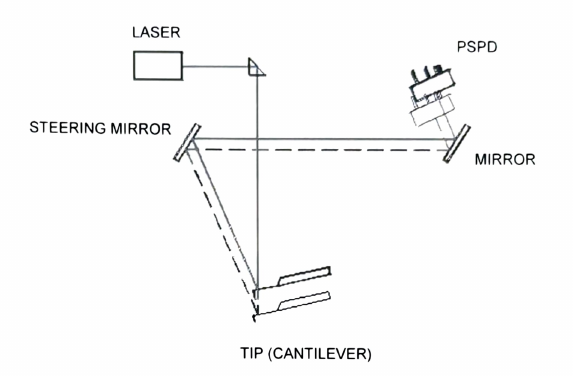
\includegraphics[width=0.6\textwidth]{../assets/messmethoden/afm/02_beam}
    \caption{Schematischer Aufbau eines Auslenkungserkennungssystems. \imcite{afm-handbuch}}
    \label{fig:afm-beam}
\end{figure}
Das System zur Auslenkungserkennung ist in \cref{fig:afm-beam} dargestellt.
Ein Laserstrahl wird aus einer Laserdiode emittiert und auf die Rückseite des Cantilevers gerichtet.
Dieser besitzt eine reflektierende Rückseite, sodass der Strahl am Cantilever zum beweglichen Spiegel reflektiert wird.
Über diesen lässt sich die Position des Strahls auf den Photodektor einstellen.
Der Strahl wird durch einen letzten Spiegel auf den Photodetektor reflektiert.


Der Photodetektor besteht aus vier Segmenten, welche in einem Quadrat angeordnet sind, wobei jedes Segment einen
Quadranten dieses Quadrats belegt.
Damit kann die Intensität des reflektierten Strahls ortsaufgelöst gemessen werden.
Im unausgelenkten Zustand muss der bewegliche Spiegel so eingestellt werden, dass der Strahl mittig auf die vier
Segmente trifft.
Kommt es zur Auslenkung, ändert sich der Winkel des Cantilevers und damit auch die Position des Strahls auf dem
Photodetektor.
Über die vier Segmente können Auslenkung und Torsion des Cantilevers bestimmt werden.

\paragraph{Feedback Controller}
Damit eine genaue Topografiekarte aufgezeichnet werden kann, ist ein schnelles und präzises Regelsystem nötig.
Durch die Regelung soll eine vorgegebene Kenngröße, beispielsweise die Auslenkung des Cantilevers, möglich konstant
gehalten werden.
Für diesen Zweck wird ein geschlossenes Regelkreissystem verwendet.
Der Regler besteht aus einem Proportional-Integral-Controller (PI-Controller), der das Fehlersignal zwischen dem
gemessenen Wert und dem Sollwert verarbeitet.
Der Proportionalanteil reagiert direkt auf den aktuellen Fehler, während der Integralanteil konstante Störungen über
die Zeit eliminiert.
Die Kombination beider Anteile ermöglicht es, sowohl kurzzeitige als auch langzeitige Abweichungen zu
korrigieren.

\paragraph{Positionierung}
Piezoelemente werden verwendet, um den Cantilever in $\mathrm{z}$-Richtung und die Probe in $\mathrm{xy}$-Richtung zu
bewegen, basierend auf dem Piezoeffekt.
Dieser Effekt tritt auf, wenn bestimmte Kristalle wie Quarz unter mechanischer Spannung elektrische Spannung erzeugen
können.
Durch Anlegen einer elektrischen Spannung an Piezokristalle können Deformationen im Bereich von \qty{0.1}{\nano\meter}
und damit in atomaren Dimensionen erreicht werden.
Spezielle Metallbiegeelemente mit eingebetteten Piezoelementen ermöglichen gezielte Verformungen, um Bewegungen
in verschiedenen Richtungen zu erzeugen.
Damit kann sowohl die Probe in $\mathrm{xy}$-Richtung, als auch der Cantilever in $\mathrm{z}$-Richtung bewegt werden.
Die Feinpositionierung und Scanbewegungen in der Rasterkraftmikroskopie werden durch Piezo-Biegeelemente gesteuert,
während eine Grobpositionsbühne für die grobe Positionierung verwendet wird.

\subsubsection{Interaktion zwischen Probe und Spitze}
Die auf die Spitze wirkende Gesamtkraft setzt sich aus verschiedenen Komponenten zusammen.
Der wichtigste und weitreichendste Beitrag entspringt der Van-der-Waals Wechselwirkung, einer attraktiven Kraft,
die durch die spontane Ausbildung fluktuierender Dipole entsteht.
Für kleinere Distanzen müssen zwei weitere Interaktionen berücksichtigt werden.
Überlappen die äußeren Elektronenhüllen von Proben- und Spitzenatomen, so können chemische Bindungen entstehen, welche
attraktive oder repulsive Kräfte hervorrufen.
Für noch kleinere Distanzen wird die Pauli-Abstoßung zwischen den Elektronen der Atome relevant.
Da die geschlossenen Elektronenschalen der Atome nicht überlappen können, müssen die zusätzlichen Elektronen auf ein
höheres Energieniveau gehoben werden.
Dadurch entsteht eine effektive repulsive Kraft.

Obwohl das System quantenmechanisch präzise beschrieben werden kann, ist die Lösung solch komplexer Systeme
nicht trivial.
Aus diesem Grund werden Modellpotentiale genutzt, die die Interaktionen zwischen Probe und Spitze approximieren.
Ein beliebtes ist das Lennard-Jones-Potential, welches sowohl die Van-der-Waals Wechselwirkung als auch die repulsiven
Anteile berücksichtigt.
\begin{equation*}
    U_{\mathrm{LJ}}=4U_{0}\left[ \left( \frac{R_{\mathrm{a}}}{r} \right)^{12} -\left( \frac{R_{\mathrm{a}}}{r}
    \right)^{6}\right]
\end{equation*}
Hierbei ist $U_{0}$ die Tiefe des Potentials, $R_{\mathrm{a}}$ der Gleichgewichtsabstand und $r$ der Abstand zwischen
den Atomen.
Das Potential ist in \cref{fig:lennard_jones} dargestellt.
Auch wenn das Lennard-Jones-Potential für atomare Wechselwirkungen entwickelt wurde, erklärt es die relevanten
Kräfte zwischen Probe und Spitze.

\begin{figure}
    \centering
    \import{../plots/messmethoden/}{lennard_jones_potential.pgf}
    \caption{Lennard-Jones-Potential.}
    \label{fig:lennard_jones}
\end{figure}

\subsubsection{Betriebsmodi}
Das Rasterkraftmikroskop verfügt über unterschiedliche Betriebsmodi.
In der vorliegenden Arbeit wurde der statische Kontaktmodus verwendet, um die Oberflächenstruktur zu erfassen.
Dabei wird die Probe in $\mathrm{xy}$-Richtung bewegt, während die Spitze des Cantilevers einen so kleinen Abstand zur
Probe hat, dass die repulsiven Kräfte dominieren.
Für den statischen Kontaktmodus liegt der Abstand im Definitionsbereich der orange dargestellten Kurve in
\cref{fig:lennard_jones}.
In diesem Bereich ist die Ableitung des Potentials negativ, was zu einer repulsiven Kraft führt.
Diese bewirkt eine Auslenkung $\Delta z$ des Cantilevers, welche durch das Erkennungssystem aufgezeichnet wird.
Mithilfe eines \textit{setpoint}-Parameters wird eine konstante Auslenkung festgelegt, die vom Feedback-System
eingehalten wird.
Scannt man über eine Erhöhung, so ändert sich die Auslenkung und das Feedback-System versucht, den Cantilever erneut
auszurichten, indem es die Höhe anpasst.
Dadurch entsteht eine Topografiekarte der Oberfläche.
Da sich die Spitze in stetigem Kontakt mit der Oberfläche befindet, müssen die Wechselwirkungskräfte
möglichst klein gehalten werden, da ansonsten die Spitze leicht kontaminiert oder beschädigt werden kann.

Nicht nur statische, sondern auch dynamische Betriebsmodi existieren.
Dabei wird der Cantilever mit einer bestimmten Frequenz und Amplitude angeregt, während er über die Probe fährt.
Ändert sich die Kraft, ändert die Resonanzfrequenz und damit auch die Amplitude.
Das Topografiesignal wird durch die Forderung einer konstanten Amplitude erzeugt.

Die in der Arbeit aufgenommenen AFM-Bilder wurden stets mit einer Scanrate von \qty{1}{\hertz}, einem
Setpoint von \num{0.4} und, bis auf eine Ausnahme, einem Scanbereich von $\qty{5}{\micro\meter} \times
\qty{5}{\micro\meter}$ aufgenommen.
Für alle Aufnahmen wurden NSC18-TI/PT Cantilever von MikroMasch verwendet.

\subsection{Weitere Messmethoden}\label{subsec:weitere-messmethoden}
Die in diesem Abschnitt vorgestellten Methoden wurden für die Arbeit verwendet, werden aber
nicht im Detail erläutert.

\paragraph{Profilometer}
Ein Profilometer ist ein Messinstrument, welches zur präzisen Messung von Oberflächenprofilen verwendet wird.
Sowohl die Topografie als auch die Rauheit der Oberfläche können bestimmt werden.
Im Gegensatz zum Rasterkraftmikroskop ist das Profilometer für gröbere Oberflächenstrukturen auf größeren Flächenskalen
ausgelegt.
Das verwendete Profilometer \textit{DektakXT} von Bruker fährt mit einer Diamantspitze über die Probe, um
die Oberflächenstruktur zu erfassen.

Die mithilfe von PLD hergestellten Dünnfilme sind durch Klemmen an den Substrathalter montiert, welche
üblicherweise kleine Regionen des Substrats, meist die Ecken, verdecken.
Da an diesen Stellen kein Dünnfilm abgeschieden wird, kann mithilfe dieser Regionen die Dicke des
Dünnfilms bestimmt werden, indem die Spitze des Profilometers sowohl über Dünnfilm als auch über eine
verdeckte Stelle fährt.
Der Höhenunterschied zwischen beiden Stellen entspricht der Dicke des Dünnfilms.

\paragraph{Energiedispersive Röntgenspektroskopie}
Eine weitere wichtige Methode zur Charakterisierung von Dünnfilmen ist die energiedispersive Röntgenspektroskopie
(EDX, engl. \textit{energy dispersive X-ray spectroscopy}), welche ortsaufgelöste chemische Kompositionsanalysen
ermöglicht.
Hierbei werden die Atome des Dünnfilms durch den Elektronenstrahl eines Rasterelektronenmikroskops (SEM, engl.
\textit{scanning electron microscope}) angeregt, welcher durch Stoßprozesse innere Elektronen aus den Atomen
herausschlägt.
Durch die anschließende Relaxation werden Röntgenstrahlen emittiert, deren Energie charakteristisch für das jeweilige
Element ist.
Die Energien der Röntgenstrahlen werden mithilfe eines Detektors aufgezeichnet und in ein Spektrum umgewandelt, welches
die Intensität in Abhängigkeit der Energie darstellt.
Da mehrere Elektronenübergänge bei der Relaxation möglich sind, entstehen in diesem Spektrum mehrere charakteristische
Peaks pro Element.
Durch die Position der Peaks können die enthaltenen Elemente ermittelt werden,
die korrespondierende Intensität gibt Aufschluss über die Konzentration der Elemente \autocite{edx}.



